
\documentclass[a4paper,12pt]{article}
\usepackage[backend=biber,sorting=none,style=gost-numeric,autolang=other]{biblatex} % библиография
%\usepackage[backend=biber,sorting=none,style=gost-numeric]{biblatex} % библиография
\usepackage{mathtext} %русские буквы в формулах
\usepackage[T2A]{fontenc}
\usepackage[utf8]{inputenc}
\usepackage[english,russian]{babel}
\usepackage{amsmath}
\usepackage{fancyvrb}
\usepackage{formular}
\usepackage{setspace} % управление междустрочными интервалами
%поля документа
\usepackage[left=3cm,right=1cm,top=2cm,bottom=2cm]{geometry}

\usepackage{misccorr} % точки в конце номеров разделов, использовать перед пакетом ccaption!
\usepackage{ccaption} % изменения подписей к рисункам и табл.

\usepackage[nooneline]{caption} 
\captionsetup[table]{justification=raggedright} % заголовок таблицы выравнивается влево
\captionsetup[figure]{justification=centering,labelsep=endash} % заголовок рисунка - по центру

% отступ перед первым абзацем
\usepackage{indentfirst}
%вставка изображений
\usepackage{graphicx}
% счетчики
\usepackage{totcount}
% управление содержанием
\usepackage{tocloft}
% управление таблицами и рисунками
\usepackage{float}

\newcounter{mycitecount}                                %% Счётчик библиографии
\AtEveryBibitem{\stepcounter{mycitecount}}              %% Работает для biblatex

\usepackage[figure,      %
            table,       %
            mycitecount, xspace ]{totalcount}           %% Подсчёт общего количества объектов в документе

% окружение для листингов - с нумерацией строк слева
\DefineVerbatimEnvironment{MyCode}{Verbatim}{frame=lines,numbers=left,numberblanklines=false,framesep=5mm}

% автоматическая нумерация листингов
\newfloat{Program}{phb}{lop}
\floatname{Program}{Листинг}
\floatstyle{ruled}

\setcounter{secnumdepth}{3} % глубина нумерации до подразделов

%если нужны точки в оглавлении для разделов - раскомментируйте следующую команду
%\renewcommand{\cftsecleader}{\cftdotfill{\cftdotsep}}

\addto\captionsrussian{%
\renewcommand{\figurename}{Рисунок}%
\renewcommand{\tablename}{Таблица}%
}

% дефис в подписи к рисункам
\captiondelim{ -- } 

% Настройки для окружений с подчеркиваниями для подписей и пр.
\setFRMfontencoding{T2A}
\setFRMdfontencoding{T2A}
% thanks to A.Starikov
\setFRMfontfamily{cmr}
\setFRMdfontfamily{ptm}
\setFRMdfontsize{10pt}

% задает длину поля для подписи на титульной странице
\newFRMfield{xtitlesign}{32mm}

% поле для факультета или кафедры
\newFRMfield{fcath}{65mm}

%имя файла с библиографией в формате BibTex
\addbibresource{rbiblio.bib}

\begin{document}

% счетчики страниц, рисунков, таблиц
\regtotcounter{page}
\regtotcounter{figure}
\regtotcounter{table}

\renewcommand{\refname}{\centerline{СПИСОК ИСПОЛЬЗОВАННОЙ ЛИТЕРАТУРЫ}} 
\renewcommand{\contentsname}{\centerline{СОДЕРЖАНИЕ}} 
%\renewcommand{\refname}{Список источников}  % По умолчанию "Список литературы" (article)
%\renewcommand{\bibname}{Литература}  % По умолчанию "Литература" (book и report)

% титульная страница
\thispagestyle{empty}
\begin{center} \small
\textbf{МИНИСТЕРСТВО ОБРАЗОВАНИЯ И НАУКИ РОССИЙСКОЙ ФЕДЕРАЦИИ}\\
ФЕДЕРАЛЬНОЕ ГОСУДАРСТВЕННОЕ АВТОНОМНОЕ ОБРАЗОВАТЕЛЬНОЕ УЧРЕЖДЕНИЕ
ВЫСШЕГО  ОБРАЗОВАНИЯ\\
«Национальный исследовательский ядерный университет «МИФИ»\\
\textbf{Обнинский институт атомной энергетики} – \\
филиал федерального государственного автономного образовательного учреждения высшего\\
образования «Национальный исследовательский ядерный университет «МИФИ»\\
(ИАТЭ НИЯУ МИФИ)
\end{center}
%\vfill
\medskip

% Направление подготовки следует уточнять,
% магистры и бакалавры могут иметь разные наименования
\begin{center}
\begin{tabular}{rl}
Отделение & \useFRMfield{fcath}[\large Интеллектуальные кибернетические системы] \\ 
Направление подготовки & \useFRMfield{fcath}[\large Информационные системы и технологии] \\ 
\end{tabular} 
\end{center}

\vfill

\large 

\begin{center}
	Научно-исследовательская работа \\
	
	\medskip
	
	\textbf{\Large 
		 Контроль электроэнергии и водоснабжения в рамках Умного города
	}
	
\end{center}

\vspace{1cm}

\begin{tabular*}{\textwidth}{lcr}
Студент группы ИС-М18 & \useFRMfield{xtitlesign} & А.В.Кузнецов\\
& & \\
Руководитель & & \\
д.т.н., профессор ОИКС & \useFRMfield{xtitlesign} & Б.И.Яцало
\end{tabular*}


\vfill
\large

\begin{center}
Обнинск, 2019 г
\end{center}

\onehalfspacing

\pagebreak

% реферат
\thispagestyle{empty}

\section*{\centering РЕФЕРАТ}

% возможно, кол-во источников придется вставлять вручную
\total{page} стр., \total{table} табл., \total{figure} рис. , \totalmycitecounts ист. 

УМНЫЙ ГОРОД, КОНТРОЛЬ РЕСУРСОВ, ИНТЕРНЕТ ВЕЩЕЙ, СИСТЕМА УЧЕТА РЕСУРСОВ, АНАЛИЗ ДАННЫХ

Настоящая работа посвящена изучению перспектив создания Умного города, разработке алгоритма поиска проблемных счетчиков электроэнергии и водоснабжения, анализу показаний квартирных и домовых приборов учета.

Разработанная система учета ресурсов позволяет жильцам получить часовые, суточные и ежемесячные данные в виде таблиц и графиков.

\pagebreak
\thispagestyle{empty}

\section*{\centering ОПРЕДЕЛЕНИЯ}
Умный город --- концепция интеграции нескольких информационных и коммуникационных технологий (ИКТ) и интернета вещей (IoT решения) для управления городским имуществом.

Интернет вещей (Internet of Things, IoT) --- концепция вычислительной сети физических предметов («вещей»), оснащённых встроенными технологиями для взаимодействия друг с другом или с внешней средой, рассматривающая организацию таких сетей как явление, способное перестроить экономические и общественные процессы, исключающее из части действий и операций необходимость участия человека. 

Геркон --- электромеханическое коммутационное устройство, изменяющее состояние подключённой электрической цепи при воздействии магнитного поля от постоянного магнита или внешнего электромагнита, например, соленоида.



\pagebreak

\section*{\centering ОБОЗНАЧЕНИЯ И СОКРАЩЕНИЯ}
\noindent
АРМ --- автоматизированное рабочее место\\
ПУ --- приборы учета\\
ПО --- программное обеспечение\\
ГВС --- Горячее водоснабжение\\
ХВС --- Холодное водоснабжение\\



\pagebreak



\tableofcontents
% если нужно добавить "Стр." над номерами страниц - раскомментируйте следующую команду
%\addtocontents{toc}{~\hfill\textbf{Стр.}\par}

\pagebreak

\section*{\centering ВВЕДЕНИЕ}
\addcontentsline{toc}{section}{ВВЕДЕНИЕ}
% введение

Термин Умный город появился относительно недавно, и определенного конкретного определения этому понятию нет. Но, все-таки  эксперты сошлись в том, что главный источник управления <<смарт сити>> – данные о населении. 

Умный город (smart city) - это стратегическая концепция по развитию городского пространства, подразумевающая совместное использование информационно - коммуникационных технологий (ИКТ) и решений Интернета вещей (IoT) для управления городской инфраструктурой. К нему относятся транспортные системы, водопроводные каналы, медицинские организации, системы переработки отходов и множество других общественных служб. \cite{Harrison}

Главная идея системы Умный город - организация информационного пространства, которое содержит в себе данные о работе контролируемых объектов (счетчиков тепловой и электрической энергии, лифтов, электротехнического оборудования, различных технических средств безопасности и т.д.). На любом расстоянии можно управлять объектами в режиме реального времени, вне зависимости от места расположения объектов и центрального управляющего пункта в городе.

Удорожание тарифов на тепловую энергию, горячую и холодную воду приводит к тому, что потребители всё больше задумываются о точной и своевременной оценке количества потреблённых ресурсов. Повсеместная установка приборов учёта является сегодня одним из приоритетных направлений реформирования ЖКХ. Однако, кроме монтажа счётчика, необходимо обеспечить возможность оперативного и регулярного снятия показаний с него. Пока счётчиков мало, эту операцию можно проводить и вручную, но как только количество узлов учёта начинает исчисляться десятками и сотнями, возникает задача создания системы автоматического сбора показаний. Такая диспетчеризация позволяет не только оперативно собирать данные, но и проводить всесторонний анализ работы теплосетей (например, выявлять неисправности).

Есть большая потребность в обработке поступающих данных в реальном времени с целью выявления аварийных и предаварийных ситуаций, нарушений работоспособности счетчиков водоснабжения, электроэнергии, нарушений режимов теплоснабжения. Такие потребности возникают и у потребителей, и у эксплуатирующих организаций, и у поставщиков тепловой энергии.

Проблема: Некорректные начисления по оплате \cite{Almanah}
\begin{itemize}
	\item Неверная работа квартирных приборов учета (неисправности, воровство); 
	\item поставка ресурсов ненадлежащего качества (недогрев, перегрев, некачественная электроэнергия);
	\item Некорректная работа регулирующего теплового оборудования; 
	\item Отсутствие технической возможности проводного соединения с квартирными приборами учета.
\end{itemize}

Решение: 
\begin{enumerate}
	\item Создание единой облачной базы данных; 
	\item Автоматизированный анализ
\end{enumerate}

\begin{itemize}
	\item Квартирные ПУ с импульсными выходами, протоколом передачи данных M-Bus, беспроводные ПУ с протоколом LoRa-WAN;
	\item Домовые электросчетчики с архивированием данных по качеству электроэнергии;
	\item Формирование базы показаний с единым форматом данных; конвертирование архивов ПУ различных производителей;
	\item Автоматизированный анализ данных.
\end{itemize}

Задачи, решаемые в ходе работы (в соответствии с заданием на НИР):
 \begin{enumerate}
 	\item Разработка автоматизированной системы учета потребления ресурсов;
	\item Анализ показаний квартирных и домовых приборов учета; 
	\item Алгоритмы поиска проблемных счетчиков электроэнергии и водоснабжения для разных типов ошибок;
	\item Описание программного обеспечения, позволяющего контролировать приборы учета.
\end{enumerate}
 % текст введения в файле intro.tex
\pagebreak

%\input{Post_zad}
\pagebreak
% первая часть

\section{Система учета ресурсов}
Система учета ресурсов предназначена для считывания, мониторинга и работы с   данными домовых счетчиков учета ресурсов. Данные со счетчиков попадают на сервер баз данных, в программе диспетчера и администратора данные отображаются, считаются, формируются отчеты. \cite{NK}

Система учета ресурсов состоит из

\begin{itemize}
	\item Сервера баз данных;
	\item Контроллеры приборов учёта;
	\item Преобразователей интерфейса;
	\item Домовой сервер (Raspberry Pi);
	\item Службы сбора данных;
	\item Управляющей программы(администратора и диспетчера).
\end{itemize}
Администратор системы должен контролировать состояния на панеле мониторинга, добавлять новые счетчики, составлять отчеты, проводить аналитику. 

Организация системы сбора показаний.

\begin{enumerate}
	\item Опросом показаний занимается программа, запущенная на домовом сервере (Raspberry Pi).  Она должна извлекать данные о требуемых к опросу счетчиках из текстового файла (приложение 1.1), производить опрос и сохранять показания в отдельный текстовый файл (приложение 1.2). Опрос показаний должен производится 1 раз  в час (например в 05 минут каждого часа).
	\item Служба сбора данных производит непосредственный опрос всех Raspberry Pi. Эта программа устанавливается на сервер баз данных и производит выгрузку файлов data.txt  с домовых серверов в единую базу данных (FireBird, PostgreSQL) (приложение 2). После занесения данных в основную базу необходимо очистить файл data.txt.  Если в основной базе изменилась информация о счетчиках (порт, адрес КПУ или номер клеммы) данная программа должна загрузить новый файл counter.txt.
	\item Раз в сутки необходимо синхронизировать время домового сервера и сервера БД (это может быть отдельная программа или одна из функций программы из п.2).	
\end{enumerate}

\textbf{квартирный учет ресурсов}
 
 В квартирном учете применена проводная система снятия показаний. Для снятия показаний приборов учета с импульсным выходом применяется универсальный счетчик СКАУТ-КПУ, поддерживающий 12 импульсных входов. Приборы с протоколами передачи данных RS485, ModBUS и другими подключаются к плате сопряжения протоколов СКАУТ

\textbf{домовой учет ресурсов}

Домовые приборы учета с импульсным выходом применяются в комплекте со счетчиком импульсов СКАУТ-КПУ. При наличии у приборов внутреннего архива, опрос приборов и промежуточное хранение файлов архива осуществляется микрокомпьютером СКАУТ-Базовый

\subsection{монтаж: установка оборудования}

\begin{enumerate}
	\item Установить комплекс СКАУТ базовый в защитный шкаф
	\item Установить контроллер приборов учета
	\item Установить "умные" счетчики, с системой телеметрии на каждый вид ресурсов (газ, электроэнергия, вода, тепло)
	\item Проложить коммутационные кабели и подключить оборудование к сети связи
	\item Установить программное обеспечение на компьютер сотрудника УК
	\item Создать базы данных по счетчикам и адресам; провести пуско-наладочные работы
	\item Провести инструктаж сотрудников УК по использованию системы учета ресурсов
\end{enumerate}  % первая глава - в файле part1.tex
\pagebreak

% вторая часть

\section{Анализ показаний приборов учета}

Учет и анализ коммунальных ресурсов дает возможность выявить их перерасход, вызванный, возможно, и халатным отношением, либо неисправностью сетей подачи ресурса. Также становится прозрачным перерасход ресурсов и несанкционированное их потребление.\cite{journal}

«Личный кабинет» программы СКАУТ позволяет получить часовые, суточные и ежемесячные данные в виде таблиц и графиков, что позволяет удобно анализировать расход ресурсов.

Детализация данных для всестороннего анализа.
Посуточная статистика. Пример приведен на рис.~\ref{fig:day}
\begin{figure}[H]
	\centering
	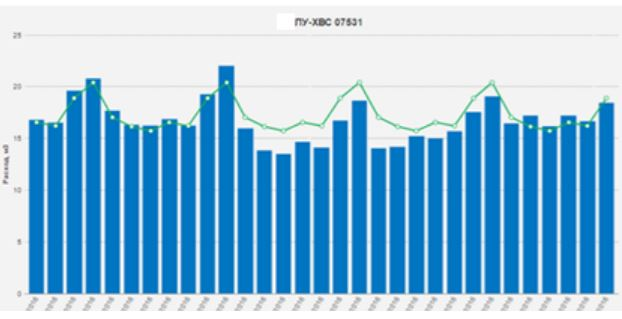
\includegraphics[width=0.7\linewidth]{pics/day}
	\caption{Посуточное потребление}
	\label{fig:day} 
\end{figure}
Почасовая статистика. Пример приведен на рис.~\ref{fig:hour}
\begin{figure}[H]
	\centering
	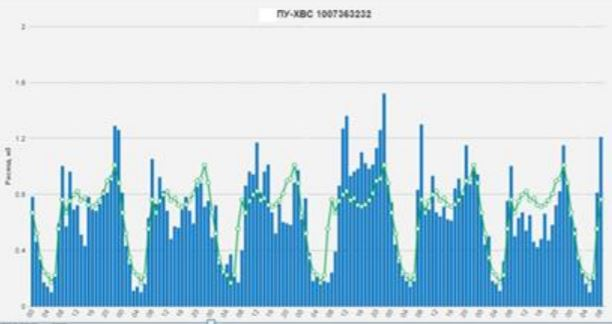
\includegraphics[width=0.7\linewidth]{pics/hour}
	\caption{Почасовые показания}
	\label{fig:hour} 
\end{figure}

С выведением информации по средне статическому потреблению.
Графическое представление, особенно за длительные сроки, даёт наглядную картину работы водосчетчиков и электросчетчиков. 

Несколько сложнее обнаруживать утечки в системе горячего водоснабжения. Непрерывный и неравномерный разбор горячей воды затрудняет их определение. Использование статистики потребления горячей воды жилым домом в ночные часы (3 часа ночи) позволяет улавливать фоновые потери для каждого дома. В основном это передавливание горячей воды в трубопровод холодного водоснабжения через неисправные квартирные смесители. Установив для каждого дома фоновый уровень потерь, можно контролировать появление протечек. До настоящего времени нами не было обнаружено таких протечек, однако данным методом в Обнинске были выявлены два 100 квартирных дома, где фоновое потребление холодной воды на дом достигало 600 литров
в час и более. В квартирах одного их них были обнаружены два неисправных сливных бачка, в другом доме протекал вентиль в подвале, и вода уходила в ливневую канализацию. После ремонтов фоновое потребление в этих домах установилось на уровне 250–300 литров в час. \cite{journal2}

Так же известно, что потребление горячей воды не может превышать потребление холодной. Данная проблема сигнализирует нам об неисправности счетчика. С помощью наложения двух графиков потребления горячей и холодной воды, можем наглядно увидеть проблемные счетчики. % вторая глава - в файле part2.tex
\pagebreak

% третья часть

\section{Алгоритмы поиска проблемных счетчиков}
Коммунальные компании постоянно сталкиваются с неучтенными расходами воды.
Чтобы справиться с утечками и сократить неучтенные расходы воды, необходимо четко представлять себе ситуацию в распределительной сети. \cite{smartcity}

Наличие нужных данных в нужное время значительно облегчает борьбу с потерей и неучтенными расходами воды и повышает эффективность этих действий. Автоматизированная система учета отображает реальное состояние распределительной сети, помогает выявить различные типы неучтенных расходов и сократить потери воды. 

Рассмотрим проблему, когда от счетчика не поступает импульс. Есть два варианта:
\begin{itemize}
	\item счетчик не исправен, по какой-то причине не крутится роликовый индикатор;
	\item счетчик работает, но импульсы от него не поступают.
\end{itemize}

Ошибка №1. Проблемы со счетчиком ХВС. 

Потребление ХВС = 0 за сутки, при этом потребление ГВС > 0 за сутки.

Алгоритм поиска:

Находим разность между показаниями счетчиков ХВС и ГВС, за текущее число и за вчерашнее.
Оставляем значения счетчиков ХВС и ГВС, где разность ХВС = 0.
Убираем значения счетчиков ХВС и ГВС, где разность ГВС = 0.

Оставшиеся счетчики ХВС являются проблемными (можно сравнивать не за сутки, а за 3 или 5).

Ошибка №2. Проблемы со счетчиком ГВС.

Потребление ГВС = 0 за неделю, при этом потребление ХВС > 0 за неделю.

Алгоритм поиска:

Находим разность между показаниями счетчиков ХВС и ГВС неделю назад и за текущее число.
Оставляем значения счетчиков ХВС и ГВС, где разность ГВС = 0.
Убираем значения счетчиков ХВС и ГВС, где разность ХВС = 0.

Получили счетчики, которые попадают в поле подозрения.
Нужно провести отбор, возможно горячей водой просто не пользуются.

Убираем счетчики, у которых значения ГВС < 5 и значение ХВС < 10.
Оставшиеся счетчики ГВС являются проблемными и требуют ручной проверки.

Ошибка №3. Проблемы со счетчиком ХВС и ГВС.

Потребление ХВС = 0, ГВС = 0 за неделю, при этом потребление Э  >= Ср.Ар. за предыдущую неделю.

Алгоритм поиска:

Находим разность между показаниями счетчиков ХВС и ГВС неделю назад и за текущее число.
Оставляем значения счетчиков ХВС и ГВС, где разность ГВС = 0 и ХВС = 0.
Находим среднее арифметическое потребление электричества за предыдущую неделю.
Если потребление электроэнергии за неделю больше чем среднее арифметическое значение, то счетчики попадают в список проблемных счетчиков.

Ошибка №4. Проблемы с электросчетчиком.

Потребление Электричества = 0 за сутки, при этом потребление ХВС > 0 и/или ГВС > 0 за сутки и более.  % третья глава - в файле part3.tex
\pagebreak

% четвертая часть

\section{Описание программного обеспечения}

Система учета ресурсов предназначена для считывания, мониторинга и работы с данными домовых счетчиков учета ресурсов. Данные со счетчиков попадают на сервер баз данных, в программе диспетчера и администратора данные отображаются, считаются, формируются отчеты.

Полный функционал программного обеспечения:
\begin{itemize}
\item управление адресами и объектами установки ПУ;
\item управление приборами учета;
\item управление абонентами; 
\item просмотр показаний ПУ за выбранный интервал времени; 
\item расчет потребления энергоресурсов по основным показаниям ПУ за указанный интервал времени; 
\item просмотр детальной информации по потреблению энергоресурсов конкретного ПУ с выводом графика потребления; 
\item предоставление сведений об аварийных и нештатных ситуациях ПУ; 
\item экспорт полученных данных в другие форматы, вывод на печать;
\item поиск.
\end{itemize}

Программа включает 9 основных разделов.
\begin{enumerate}
	\item Раздел - Показания приборов
	\item Раздел - Состояние приборов учета
	\item Раздел - Адреса
	\item Раздел - Абоненты
	\item Раздел - Приборы учета
	\item Раздел - Лицевые счета
	\item Раздел - Отчеты
	\item Раздел - Поиск
	\item Раздел - Оповещение об ошибках и нештатных ситуациях
\end{enumerate}

Система должна быть защищенной и поэтому используются локальные данные. Сервер, база данных на постгрессе и программы на компьютерах администраторов для управления. 

\textbf{Цели:} Сбор данных и мониторинг потребления ресурсов.
 
\textbf{Задачи:}  Создать защищенную и удобную систему  для сбора данных потребляемых населением.

Программа для администратора: мониторинг, добавление/ изменение/ удаление счетчиков, составление отчетов. 

Функции программы диспетчера:

Ведение списка пользователей и управление их полномочиями;
Конфигурация для сохранения, изменения и отображать данных о подключении счетчика к конкретной КПУ (порт, адрес, клемма, коэффициент- цены импульса). 
\begin{itemize}
	\item Ведение служебных справочников (список адресов, типов приборов и т.д.);
	\item Ввод и редактирование данных о подключенных контроллерах;
	\begin{enumerate}
		\item Создание прикрепленных индивидуальных приборов учёта с указанием:
		\begin{enumerate}
			\item номера клеммы; 
			\item цены импульса; 
			\item типа прибора;
			\item серийного номера; 
			\item единиц измерения;
			\item начального показания;
			\item номера квартиры;
			\item ФИО собственника;
		\end{enumerate}
		\item Для счётчиков требующих проверки указать дату предыдущей и следующей поверки;
		\item Групповые операции с устройствами;
	\end{enumerate}
	\item Просмотр показаний приборов учёта в табличном и графическом виде;
	\begin{enumerate}
		\item Отображение сведений о наличии или отсутствии показаний за выбранный период для выбранных устройств;
	\end{enumerate}
	\item Формирование отчетов по потреблению ресурсов – ежемесячный отчет установленного формата для управляющей компании/ресурсоснабжающей организации;
	\item Сравнение суммарного квартирного потребления и общедомового (при наличии возможности).
	
\end{itemize} % четвертая глава - в файле part4.tex
\pagebreak

%\input{part5}  % пятая глава - в файле part5.tex
%\pagebreak

\section*{\centering ЗАКЛЮЧЕНИЕ}
\addcontentsline{toc}{section}{ЗАКЛЮЧЕНИЕ}
В России интерес к тематике Умного города растет с каждым годом, в том числе потому, что многие города подходят к пределам надежности и функциональности существующей инфраструктуры.

Разработана автоматизированная система учета потребления ресурсов.

Проведен анализ показаний квартирных и домовых приборов учета.

Рассмотрены основные алгоритмы поиска проблемных счетчиков электроэнергии и водоснабжения для разных типов ошибок.

Описано программное обеспечение для управления ресурсами электроэнергии и водоснабжения.

В связи с тем, что большинство современных счетчиков поддерживает протокол ModBus, появилась возможность усовершенствования системы и переноса отработанных алгоритмов анализа на web-платформу. Также планируется реализация новых задач анализа данных.

% оформление библиографии - вариант с БД
\pagebreak

\addcontentsline{toc}{section}{СПИСОК ИСПОЛЬЗОВАННОЙ ЛИТЕРАТУРЫ}
% ВАЖНО: для корректного отображения в списке литературы ссылок на англ.языке в bibtex-описание источника следует добавить поле 
% langid = {english}
\printbibliography

\pagebreak

\section*{ \centering Приложение 1} 
\addcontentsline{toc}{section}{Приложение 1}

\begin{center}
	Формат текстовых данных на домовом сервере
\end{center}

\subsection*{1.1 Формат файла данных о счетчиках}
Файл представляет собой CSV файл (разделение символом ; ). Название counters.txt
Поля:
\begin{enumerate}
	\item Порт компьютера;
	\item Адрес КПУ на шине;
	\item Номер клеммы;
\end{enumerate}
Пример: /dev/ttyUSB0;05;3

\subsection*{1.2 Формат файла данных с показаниями}
Файл представляет собой CSV файл (разделение символом ; ). Название data.txt
Поля:
\begin{enumerate}
	\item Порт компьютера;
	\item Адрес КПУ на шине;
	\item Номер клеммы;
	\item Дата;
	\item Время (час без указания минут);
	\item Показание.
\end{enumerate}
Пример: /dev/ttyUSB0;05;3;10.10.2017;12;34.5

\pagebreak

\section*{ \centering Приложение 2} 
\addcontentsline{toc}{section}{Приложение 2}

\begin{center}
	База данных на сервере данных
\end{center}

\subsection*{2.1 Концептуальная схема БД}
\begin{figure}[H]
	\centering
	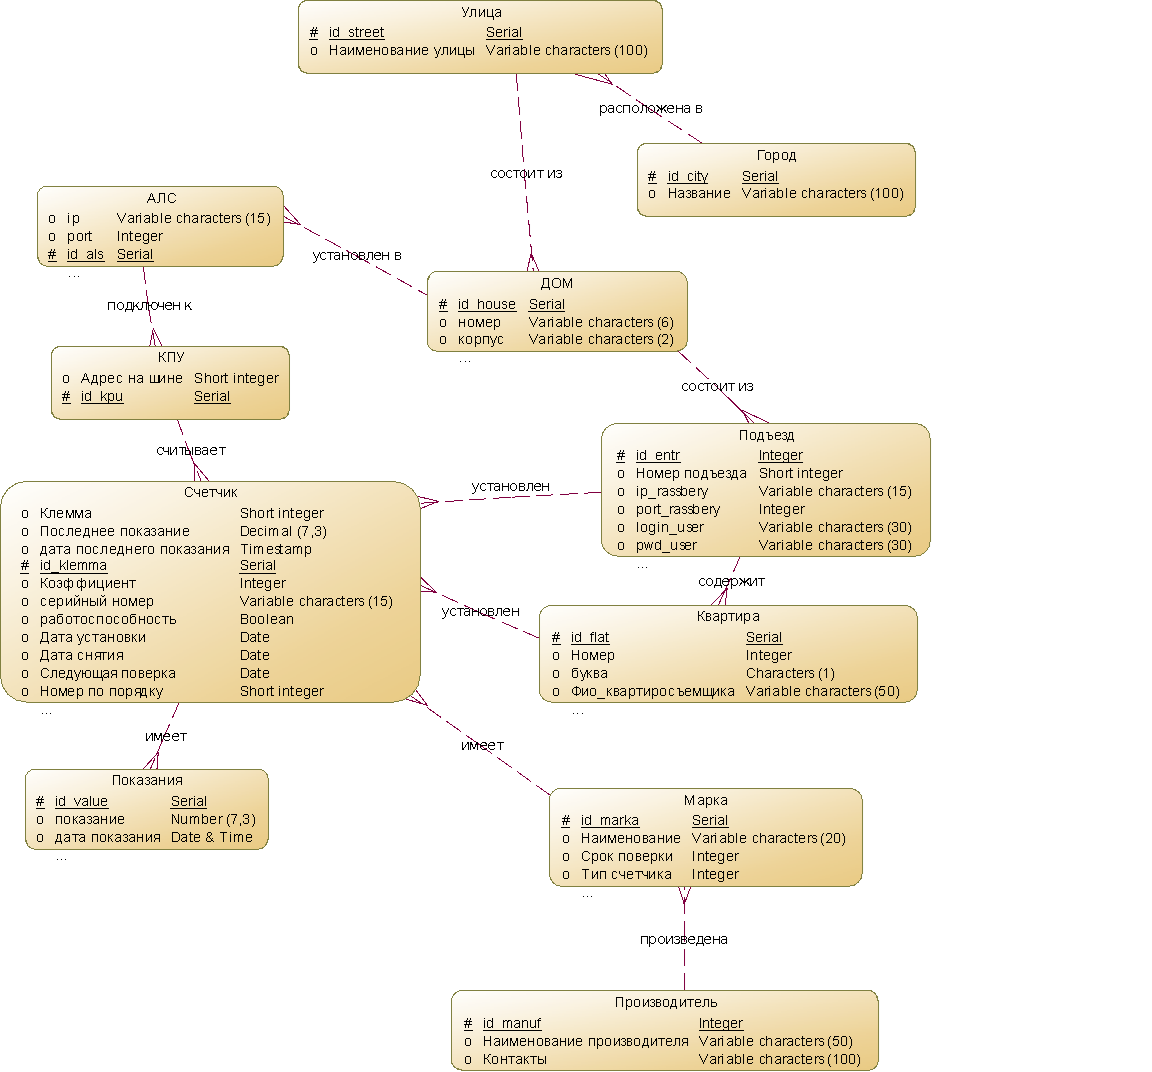
\includegraphics[width=1.2\linewidth]{pics/pril1} 
\end{figure}

\pagebreak

\subsection*{2.2 Физическая схема БД}
\begin{figure}[H]
	\centering
	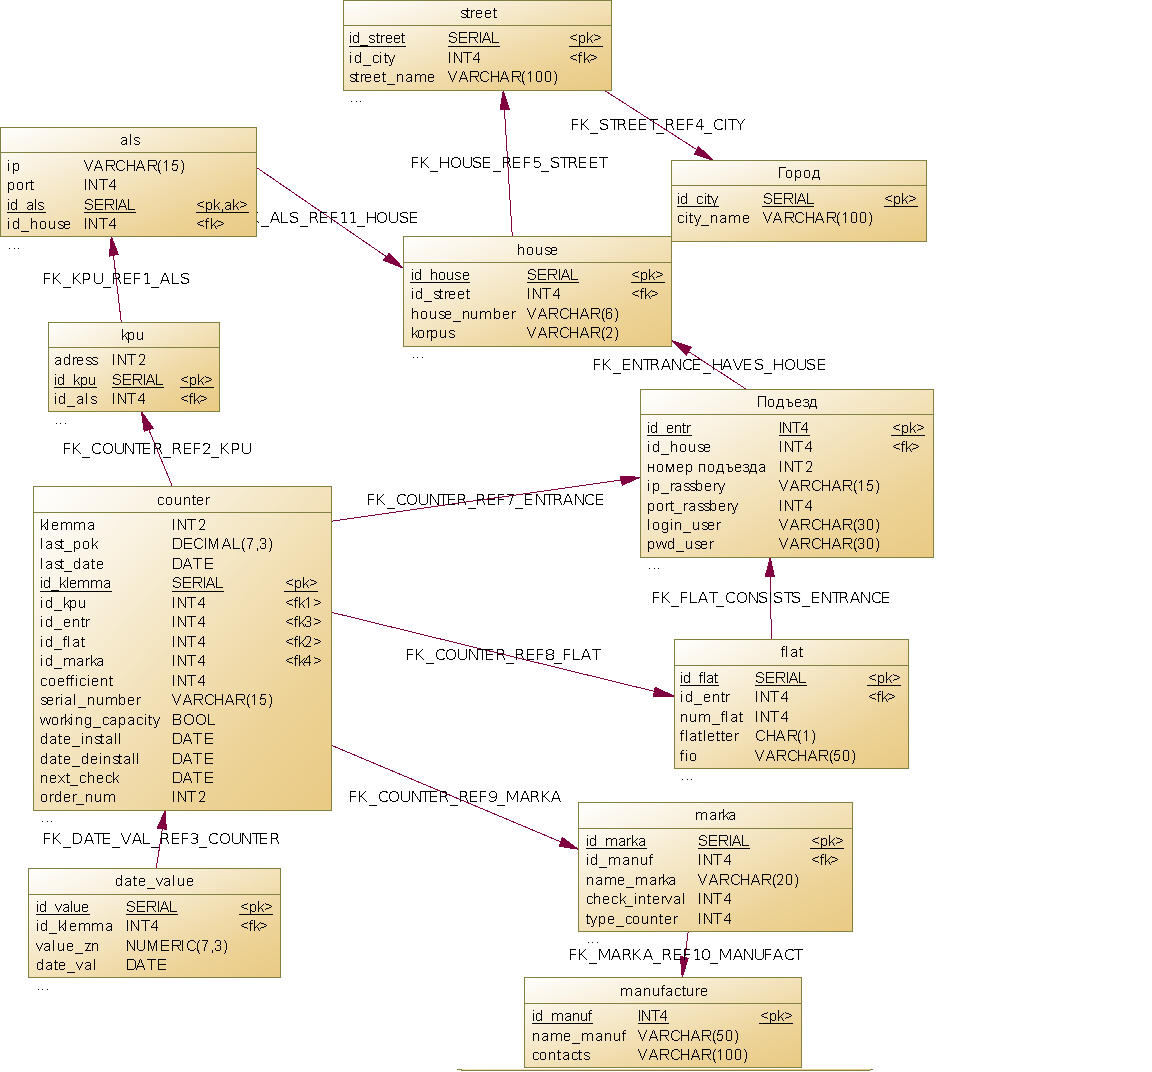
\includegraphics[width=1.2\linewidth]{pics/pril2} 
\end{figure}

\end{document}          

